\chapter{Gitterprobleme}\label{ch:lattice_problems}

Die Struktur von Gittern verleiht ihnen besondere mathematische Eigenschaften. Es gibt \glqq einfache\grqq{} Gitterprobleme, die sich mit den Werkzeugen der linearen Algebra lösen lassen. Von anderen Gitterproblemen glaubt man, dass sie NP-schwer und resistent gegen den Algorithmus von Shor sind, und damit quanten-resistent.

\section{Ein einfaches Gitterproblem}
Gegeben sind Vektoren $\mathbf{g}_1, \dots, \mathbf{g}_k \in \mathbb{R}^n$, die ein Gitter $\mathcal{L}$ erzeugen. Gesucht ist eine Basis $\mathbf{b}_1, \dots, \mathbf{b}_m$ von $\mathcal{L}$. Zusätzlich soll entschieden werden, ob ein beliebiger Vektor $\mathbf{c}$ in $\mathcal{L}$ liegt.

\textbf{Lösungsansatz:}
\begin{enumerate}
    \item Aus den $\mathbf{g}_i$ mit dem Gauss-Algorithmus eine Basismatrix $\mathbf{B}$ berechnen.
    \item Das lineare Gleichungssystem $\mathbf{B}\mathbf{x} = \mathbf{c}$ lösen.
    \item $\mathbf{c}$ ist genau dann ein Element von $\mathcal{L}$, wenn $\mathbf{x} \in \mathbb{Z}^m$ gilt (alle Einträge ganzzahlig).
\end{enumerate}

Das Gitter besteht per Definition aus allen ganzzahligen Linearkombinationen der Basisvektoren, also $\mathcal{L} = \{\mathbf{B}\mathbf{x} : \mathbf{x} \in \mathbb{Z}^m\}$. Da die Basisvektoren linear unabhängig sind, hat $\mathbf{B}\mathbf{x} = \mathbf{c}$ höchstens eine Lösung. Ist sie nicht ganzzahlig, gibt es keine andere, ganzzahlige Darstellung von $\mathbf{c}$.

\section{Shortest Vector Problem (SVP)}
Vereinfacht gesagt ist das SVP die Suche nach dem Gittervektor mit der kürzesten Distanz zum Ursprung.

\begin{definition}[Shortest Vector Problem (SVP)]
    Sei $\mathcal{L}$ ein Gitter mit einer Basis $\mathbf{B} \in \mathbb{R}^{n \times m}$ und einer Norm $\|\cdot\|$. Sei $\lambda(\mathcal{L})$ die Länge des kürzesten Vektors ungleich null in $\mathcal{L}$. Die Aufgabe, ein $\mathbf{l} \in \mathcal{L}$ zu finden mit $\|\mathbf{l}\| = \lambda(\mathcal{L})$, also irgendeinen kürzesten Vektor von $\mathcal{L}$ zu finden, heisst \textit{Shortest Vector Problem (SVP)}.
\end{definition}

\begin{figure}[H]
    \centering
    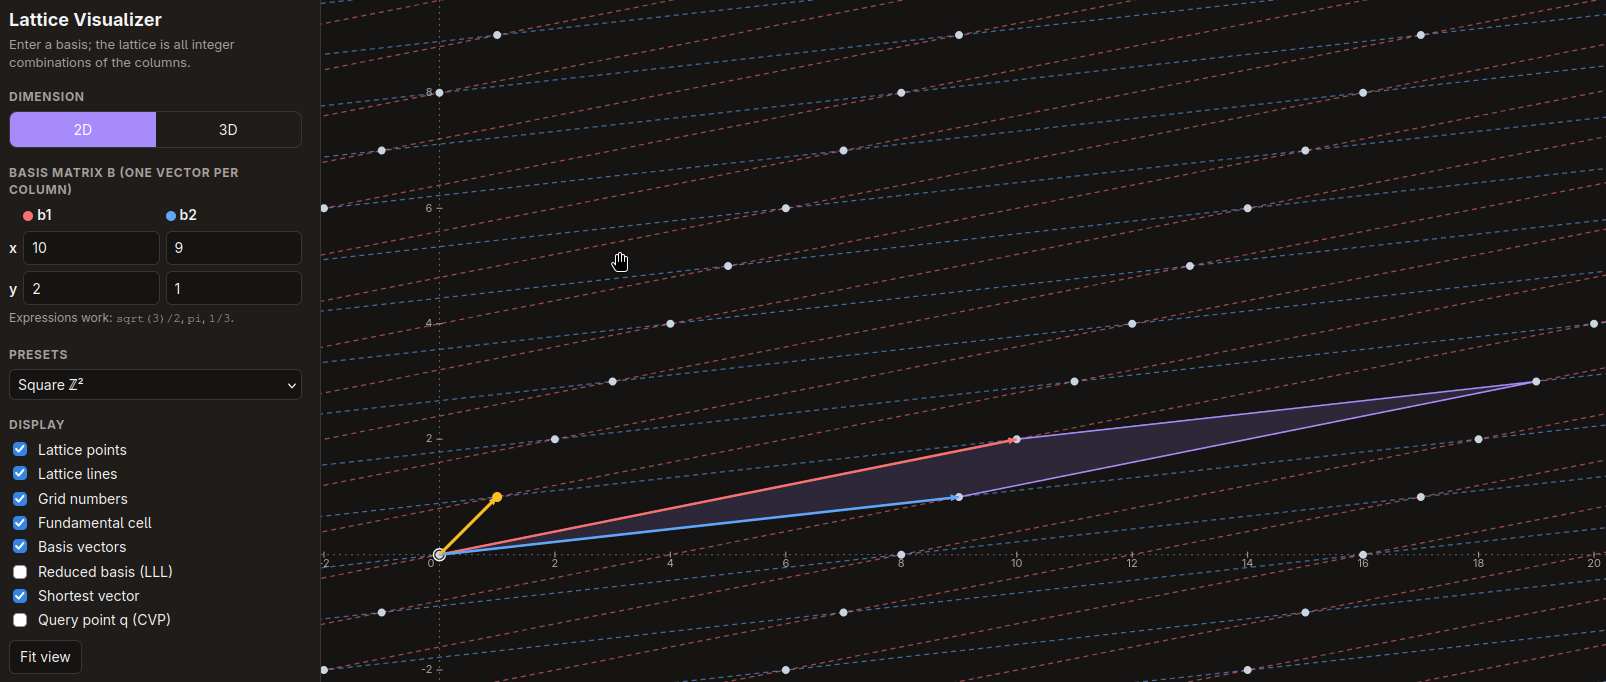
\includegraphics[width=0.9\textwidth]{../assets/lattice_tool_shortest_vector_problem.png}
    \caption{Der kürzeste Vektor eines Gitters}
\end{figure}

SVP ist NP-schwer. Die besten exakten Algorithmen brauchen exponentielle Zeit in der Dimension $n$, z.B. Enumeration in $2^{O(n \log n)}$.

\section{Closest Vector Problem (CVP)}
Die Suche nach dem Gittervektor mit der kürzesten Distanz zu einem beliebig gewählten Punkt heisst \textit{Closest Vector Problem (CVP)}.

\begin{definition}[Closest Vector Problem (CVP)]
    Sei $\mathcal{L}$ ein Gitter mit einer Basis $\mathbf{B} \in \mathbb{R}^{n \times m}$ und einer Norm $\|\cdot\|$. Gegeben sei ein $\mathbf{q} \in \mathbb{R}^n$. Die Aufgabe, ein $\mathbf{l} \in \mathcal{L}$ zu finden, für das $\|\mathbf{l} - \mathbf{q}\|$ minimal ist, heisst \textit{Closest Vector Problem (CVP)}.
\end{definition}

\begin{figure}[H]
    \centering
    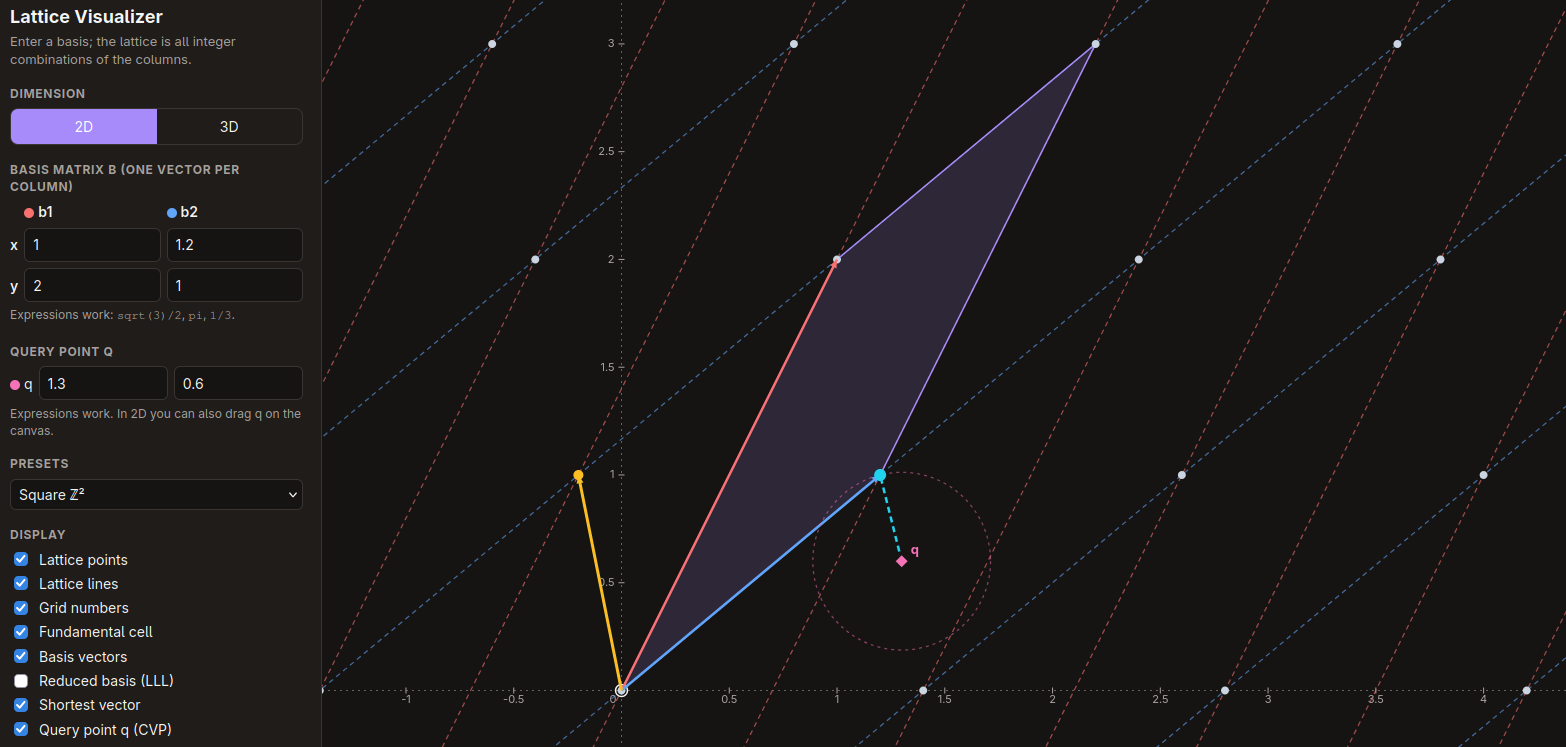
\includegraphics[width=0.9\textwidth]{../assets/lattice_tool_closest_vector_problem.png}
    \caption{Der nächstgelegene Gittervektor zu einem Punkt $\mathbf{q}$}
\end{figure}

CVP ist NP-schwer und gilt als mindestens so schwer wie SVP.
